\subsection{UCD\textbf{Noch nicht überarbeitet!}}

Durch den schnellen Wandel der Technik in den vergangenen Jahrzehnten, haben sich Systeme sehr stark weiterentwickelt. Vor allem durch das Smartphone und neuerdings auch Smarthome Produkte sind in unserem Alltag fest verankert. Bloß haben beide 'Systeme' nicht zu viel mit dem Auto \textit{(wie man es heute kennt)} zu tun - bis jetzt.\\
Diese beiden Produktarten sind Beispiele für Alltagsunterstützer, Geräte die uns alltäglich begleiten und uns einiges an Arbeit abnehmen. Das 'Auto' hingegen passt eher wenig an den Fahrer an. Zwar gibt es viele elektronische Assistenzsysteme (Sitzverstellung z.B.) und mittlerweile auch Schnittstellen, um unser Handy mit dem Fahrzeug zu verbinden - aber das Auto selber agiert in der Regel noch nicht individuell mit dem Fahrer.\\
Auch wenn die bisherigen Systeme ihre Aufgabe gut gemacht haben, gibt es einen gravierenden Unterschied zu einem Produkt wie dem Smartphone und zwar die Ausreizung der Usability sowie der User Experience des jeweiligen Systems. Sogenanntes Human-Centered-Design\cite{b23} (oder auch User Centered Design) bezieht den letztendlichen Nutzer in den Designprozess des Systems mit ein. Hierdurch wird direkte Kommunikation von den Nutzern an die Entwickler und umgekehrt geschaffen. Der Ablauf von User-Centered-Design ist in 4 Zyklen aufgeteilt: (Zitat)\\


\fbox{\begin{minipage}[c]{42em}
Vgl. hier\cite{b24}
"
\begin{itemize}
	\item \textit{\textbf{Analyse}}\\
	\textit{Diese Phase stellt sicher, dass alle Geschäfts- und Benutzeranforderungen vor Beginn der Entwurfsphase berücksichtigt werden. Konkrete Aufgaben während dieser Phase sind die Stakeholder-, Nutzer- und Zielgruppenanalyse inklusive der Beurteilung von Erfahrung und Fähigkeiten der zukünftigen Nutzer, die Entwicklung von Personas und die Definition der Benutzerszenarien. Weiterhin sind die Definition der Usability Ziele, die Festlegung von Messungen und Testzielen sowie gegebenenfalls die Durchführung von Feldstudien Bestandteil der Analyse.}
	\item \textbf{Konzeption}\\
	\textit{Die Konzeptionsphase des User-Centered Design ist eine Synthesephase, die darauf abzielt, das Verständnis für die Benutzer und deren Bedürfnisse hinsichtlich der User Experience auf das Design der Benutzeroberfläche oder der Webseite zu übertragen. Der Zweck dieser Phase besteht darin, die Benutzerinteraktion mit dem zukünftigen System zu definieren, ohne es zu entwerfen. Die verschiedenen Anwendungsszenarien, die bereits in der Analysephase entwickelt wurden, werden in Task Flows und Storyboards detailliert beschrieben. Zusätzlich werden häufig Wireframes erstellt, die in Form eines anklickbaren Prototyps geliefert werden können und von Endbenutzern getestet werden, um sicherzustellen, dass die geplante Anwendung ihren Anforderungen entspricht.}
	\item \textbf{Design}\\
	\textit{Die Design Phase dient beim User-Centered Design keinem Selbstzweck. Sie sollte vielmehr als Möglichkeit betrachtet werden, Probleme zu lösen und eine optimale User Experience sicherzustellen. Ein konsistentes, ansprechendes und klares Grafik Design hilft dabei, eine Marke zu stärken, Informationen auf sinnvolle Weise zu präsentieren und die Benutzererfahrung durch die Erstellung einer intuitiv nutzbaren Oberfläche zu verbessern.}
	\item \textbf{Evaluierung \& Optimierung}\\
	\textit{Nachdem das Produkt erstellt wurde sowie kurz vor dessen Veröffentlichung werden Usability-Tests mit Benutzern durchgeführt, um den Erfolg des Produkts und die User Experience zu bewerten. Der Erfolg kann beispielsweise mit dem Usability Key Performance Indicator (KPI) gemessen werden. Hierbei werden Effektivität (d.h. wie gut das System es dem Benutzer ermöglicht, seine Ziele zu erreichen) sowie Effizienz (wie viel Aufwand und Zeit erforderlich ist, um Aufgaben auszuführen) getestet. Hinzu kommen je nach Produkt weitere Tests, die zeigen, wie hoch die Nutzungssicherheit ist, d.h. inwiefern eine Umgebung einschließlich der Geräte, Software, Einrichtungen oder Personen frei von Gefahren ist. Nicht zuletzt werden die Zufriedenheit der Nutzer, ihre subjektive Wahrnehmung sowie ihre Reaktionen ermittelt.}\\
	
	\textit{Zeigen sich bei der Evaluierung Mängel, wird das Design entsprechend überarbeitet und das Produkt erneut evaluiert. Wenn die gestellten Anforderungen und die Qualitätsansprüche erfüllt sind, kann das Produkt ausgeliefert werden. Stellt sich heraus, dass der Informationsstand diesbezüglich nicht ausreichend ist, müssen gegebenenfalls weitere Analysen durchgeführt werden. Dieses Vorgehen hilft beim User-Centered Design dabei, Fehler zu vermeiden, die ansonsten erst nach der Auslieferung des Produktes an die Nutzer entdeckt werden und dann nur mit erheblichem Mehraufwand zu beheben sind.}
	
\end{itemize}
"
\end{minipage}
}
\clearpage
Und hier zur Übersicht der Kreislauf des User-Centered-Designs\\
\begin{figure}[!h]
	\centering
	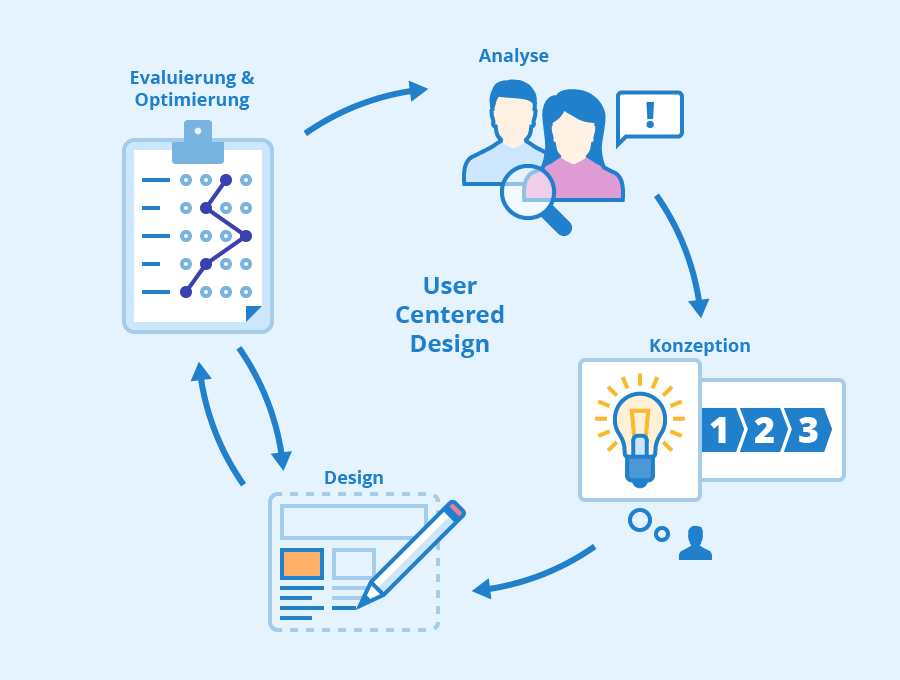
\includegraphics[width=0.734\columnwidth]{pictures/ucd.png}
	\caption{ User Centered Design - Autor: Seobility}
	\label{img:ucd}
\end{figure}
Der US-Amerikanische Wissenschaftler des "Massachusetts Institute of Technology", Lex Fridman, beschäftigte sich unter anderem mit den Aufstellen von Richtlinien für das entwickeln von sogenannten "Human \textit{(User)} Centered Vehicles".\\
Durch den Wandel der Wirtschaft zu einem Nachfrageorientierten Markt müssen Unternehmen dem Kunden viele neue Mehrwerte bieten, um diese von einem Kauf zu überzeugen. Grade das Smartphone 